\documentclass[border=0.5cm]{standalone}
\usepackage{tikz}
\usepackage{amsmath}
\usetikzlibrary{calc, angles, quotes}

\begin{document}
\begin{minipage}{.6\textwidth}
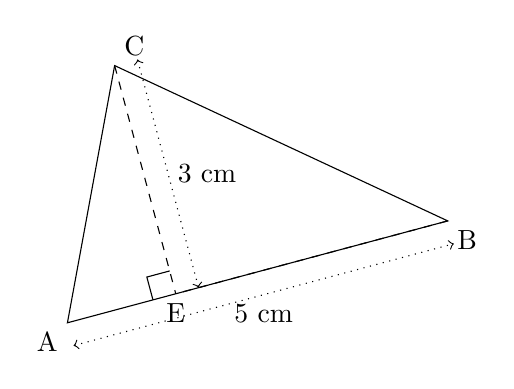
\begin{tikzpicture}
    \begin{scope}[rotate=15]
    \coordinate (A) at (0,0);
    \draw (A) -- ++(5,0) coordinate (B) -- ++(140:{3/sin(140)}) coordinate (C) -- cycle; % Removed the line to D
    \coordinate (E) at ($(C) + (0,-3)$);
    \draw[dashed] (B) -- (E);
    \draw[dashed] (C) -- (E);
    \pic [draw, -, angle radius=0.3cm, angle eccentricity=1.6] {right angle=C--E--A};
    
    \foreach \point/\position in {A/below left, B/below right, C/above right, E/below} { % Removed D
        \node[\position] at (\point) {\point};
    }
    
    % Add arrows to indicate lengths
    \draw[<->, dotted] ($(A)!0.0!(B)$) ++(-0.0cm,-0.3cm) -- ++(5cm,0) node[midway,below] {5 cm};
    \draw[<->, dotted] ($(C)!0.0!(E)$) ++(0.3cm,-0.0cm) -- ++(0,-3cm) node[midway,right] {3 cm};
    
    \end{scope}
\end{tikzpicture}
\end{minipage}%
\begin{minipage}{.4\textwidth}
\begin{align*}
\text{Area} &= \frac{1}{2} \text{bh} \\ % Changed formula to triangle area formula
\text{Area} &= \frac{1}{2} \times 5 \text{cm} \times 3 \text{cm}  \\ % Changed values to match triangle dimensions
\text{Area} &= 7.5 \text{cm}^2 % Updated area value
\end{align*}
\end{minipage}

\end{document}
